\documentclass[12pt,fullpage,letterpaper]{article}

\newenvironment{proof}{\noindent{\bf Proof:}}{\qed\bigskip}

\newtheorem{theorem}{Theorem}
\newtheorem{corollary}{Corollary}
\newtheorem{lemma}{Lemma} 
\newtheorem{claim}{Claim}
\newtheorem{fact}{Fact}
\newtheorem{definition}{Definition}
\newtheorem{assumption}{Assumption}
\newtheorem{observation}{Observation}
\newtheorem{example}{Example}
\newcommand{\qed}{\rule{7pt}{7pt}}


\newcommand{\assignment}[4]{
\thispagestyle{plain} 
\newpage
\setcounter{page}{1}
\noindent
\begin{center}
\framebox{ \vbox{ \hbox to 6.28in
{\bf CS6501: Advanced Machine Learning \hfill #1}
\vspace{4mm}
\hbox to 6.28in
{\hspace{2.5in}\large\mbox{Problem Set #2}}
\vspace{4mm}
\hbox to 6.28in
{{\it Handed Out: #3 \hfill Due: #4}}
}}
\end{center}
}

\newcommand{\handout}[3]{
\thispagestyle{plain} 
\newpage
\setcounter{page}{1}
\noindent
\begin{center}
\framebox{ \vbox{ \hbox to 6.28in
{\bf CS6501-01 Advanced Machine Learning  \hfill #1}
\vspace{4mm}
\hbox to 6.28in
{\hspace{2.5in}\large\mbox{#2}}
\vspace{4mm}
\hbox to 6.28in
{{\it Date: #3 \hfill Name (NetID):\makebox[2in]{\hrulefill}}}
}}
\end{center}
}

\newcommand{\solution}[4]{
\thispagestyle{plain} 
\newpage
\setcounter{page}{1}
\noindent
\begin{center}
\framebox{ \vbox{ \hbox to 6.28in
{\bf CS6501 - Advanced Machine Learning \hfill #4}
\vspace{4mm}
\hbox to 6.28in
{\hspace{2.5in}\large\mbox{Problem Set #3}}
\vspace{4mm}
\hbox to 6.28in
{#1 \hfill {\it Handed In: #2}}
}}
\end{center}
\markright{#1}
}

\newenvironment{algorithm}
{\begin{center}
\begin{tabular}{|l|}
\hline
\begin{minipage}{1in}
\begin{tabbing}
\quad\=\qquad\=\qquad\=\qquad\=\qquad\=\qquad\=\qquad\=\kill}
{\end{tabbing}
\end{minipage} \\
\hline
\end{tabular}
\end{center}}

\def\Comment#1{\textsf{\textsl{$\langle\!\langle$#1\/$\rangle\!\rangle$}}}


\usepackage{graphicx}
\usepackage{subfigure}
\usepackage{amsmath}
\usepackage{amssymb}
%\usepackage{qtree}
\usepackage{epsfig}
\usepackage{enumerate}
\usepackage{color}
\usepackage{algorithmic}
\usepackage{hyperref}

%\usepackage{parskip}

\sloppy
\parskip = 0.5cm

\newcommand{\ignore}[1]{}
\newcommand{\pp}{\noindent}
\newcommand{\ov}{\overline}
\newcommand{\bb}[1]{{\bf #1}}
\renewcommand{\labelitemii}{\tiny$\circ$}

\newcommand{\question}[1]{#1}%{}
%\newcommand{\answer}[2]{#1}
%\input{answerdef.tex}
%\newcommand{\answer}[2]{#1}
\newcommand{\answer}[2]{{
\vspace{10pt} 
\color{red}{#2}
\vspace{10pt}
}
}
\newcommand{\comment}[1]{}


\oddsidemargin 0in
\evensidemargin 0in
\textwidth 6.5in
\topmargin -0.5in
\textheight 9.0in

\begin{document}
\setlength{\unitlength}{1mm}

\thispagestyle{plain}
\newpage
\assignment{2017}{3}{April 18, 2017}{April 26, 2017}

\begin{itemize}
\item Feel free to talk to other members of the class in doing the homework. You should, however,
write down your solution yourself.  Please try to keep the solution brief and clear.

\item Please use Piazza first if you have questions about the homework. Also feel free to come to office hours.

\item Please, no handwritten solutions. You will submit your solution manuscript as a single pdf file. Please use \LaTeX to typeset your solutions.

\item The homework is due at 11:59 PM on the due date. We will be using
Collab for collecting the homework assignments. Please submit your solution manuscript as a pdf file.  Please do NOT hand in a hard copy of your write-up.
Contact the TAs if you are having technical difficulties in 
submitting the assignment. 
\end{itemize}



\section{Augmented Inference for Sequential Tagging Models} 

In this problem set, let's derive a loss-augmented Viterbi algorithm for sequential tagging. We assume the scoring function $w^T \phi(x,y)$ can be decomposed based on the following factor graph (i.e.,  $w^T \phi(x,y)= \sum_{i=1}^{n} w^T\phi(x,y_{i-1}, y_i)$. The output structure is $y=y_1, y_2, y_3, \ldots, y_n$, where each output variable can take a value from 1 to m (i.e., $y_i\in \{1,2,\ldots m\})$.) $w^T\phi(x,y_{i-1}, y_i)$ is the score assigned to the factor $(x,y_{i-1}, y_i)$ by a model $w$.

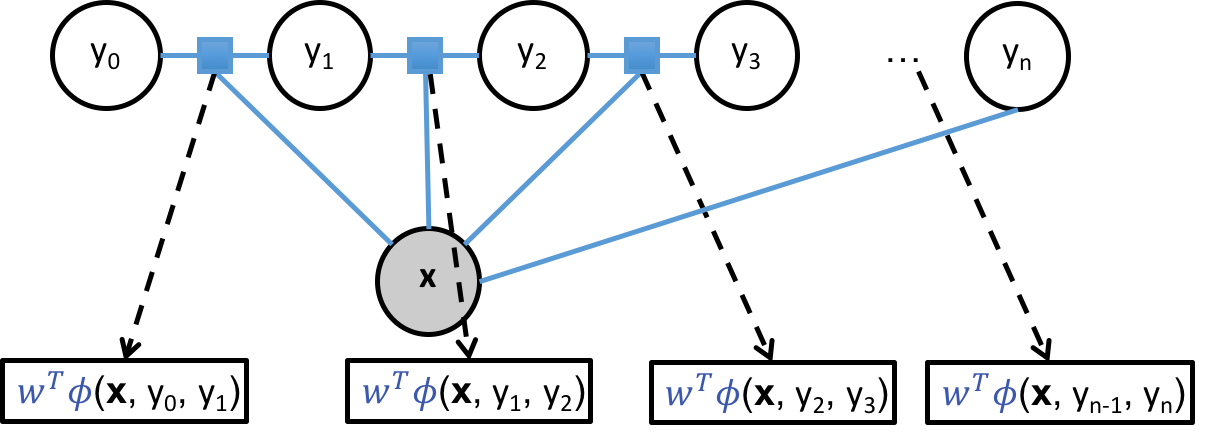
\includegraphics[width=0.8\linewidth]{factor}



\begin{itemize}
\item[{\bf Question A}][20points]: Write down an efficient algorithm for computing $\max_{y} w^T \phi(x,y)$ in $O(nm^2)$ time. Hint:  look at Hw2 solution (\url{http://www.cs.virginia.edu/~kc2wc/teaching/SL17/hw2_solution.pdf}). In that problem, we ask to design an algorithm for sum-product inference. Here, we are looking for an algorithm for max-sum inference.)

\item[{\bf Question B}][20points]:  Assume $\Delta(y,y')$ is the Hamming loss (the number of labels in the sequence that are incorrectly predicted). Please write down an algorithm for the loss-augmented inference algorithms. Hint: Recall that in lecture 9 (\url{http://www.cs.virginia.edu/~kc2wc/teaching/SL17/09-learning.pdf}), page 61. We show an example of how to include Hamming loss in the inference problem. 

\end{itemize}


\section{Belief Propagation} 
In Lecture 8 (\url{http://www.cs.virginia.edu/~kc2wc/teaching/SL17/08-inference.pdf}, we discuss belief propagation algorithms.  We assume the global score $f(x)$ is factorized into $f(x)=\Pi_{i}g_i(x_i)\Pi_{i,j}f_{ij}(x_i,x_j)$. The max-product inference algorithm can be used to estimate
$\max f(x)$. However, in many cases, calculating $\max f(x)$  encounters a numerical problem (either overflow or underflow). Therefore, we should compute $\max \log f(x)$ instead. That is, we want to design an algorithm to evaluate the following max-sum inference
$$\max \sum_{i}\log g_i(x_i) + \sum_{i,j} \log f_{ij}(x_i,x_j)$$
\begin{itemize}
\item[{\bf Question A}][10points]: Write down the message update rule. ($m_{ij}^{new}(x_j)= \ldots$) Hint: 
see page 79.

\item[{\bf Question B}] [0point]:
In page 81-104 we show examples of the sum-product and the max-product inference algorithms. The former is usually used to compute the partition function, and the latter is used to find the best output assignment. Make sure you understand these algorithms and try out a max-sum inference algorithm on this example.
\end{itemize}

\end{document}
